%% LyX 2.3.0 created this file.  For more info, see http://www.lyx.org/.
%% Do not edit unless you really know what you are doing.
\documentclass[american]{beamer}
\usepackage{mathptmx}
\usepackage[T1]{fontenc}
\usepackage[latin9]{inputenc}
\setcounter{secnumdepth}{4}
\setcounter{tocdepth}{1}
\usepackage[active]{srcltx}
\usepackage{array}
\usepackage{booktabs}
\usepackage{amsmath}
\usepackage{amssymb}
\usepackage{graphicx}

\makeatletter

%%%%%%%%%%%%%%%%%%%%%%%%%%%%%% LyX specific LaTeX commands.
%% Because html converters don't know tabularnewline
\providecommand{\tabularnewline}{\\}

%%%%%%%%%%%%%%%%%%%%%%%%%%%%%% Textclass specific LaTeX commands.
% this default might be overridden by plain title style
\newcommand\makebeamertitle{\frame{\maketitle}}%
% (ERT) argument for the TOC
\AtBeginDocument{%
  \let\origtableofcontents=\tableofcontents
  \def\tableofcontents{\@ifnextchar[{\origtableofcontents}{\gobbletableofcontents}}
  \def\gobbletableofcontents#1{\origtableofcontents}
}

%%%%%%%%%%%%%%%%%%%%%%%%%%%%%% User specified LaTeX commands.
\usetheme{Warsaw}
% or ...

\setbeamercovered{transparent}
% or whatever (possibly just delete it)

\makeatother

\usepackage{babel}
\begin{document}

\title[Analyzing the Brazilian Formal Labor Market w/ GVAR]{Modeling How Macroeconomic Shocks Affect Regional Employment: Analyzing
the Brazilian Formal Labor Market using the Global VAR Approach}

\author[Barbosa, Mar�al - Sao Paulo School of Economics ]{Bruno Tebaldi de Queiroz Barbosa\\
Emerson Fernandes Mar�al\\
}

\institute[emerson.marcal@fgv.br]{Sao Paulo School of Economics, FGV \\
20th OxMetrics User Conference\\
}

\makebeamertitle
%\pgfdeclareimage[height=0.5cm]{institution-logo}{cemap_logo}


%\logo{\pgfuseimage{institution-logo}}

\pgfdeclareimage[height=1.5cm]{institution-logo}{logo-conjunto.png}


%\pgfdeclareimage[height=1.5cm]{institution-logo}{C:\Users\emerson.marcal\Dropbox\FGV\CEMAP\pesquisas\observatorio\TB-NFA-approach\apresentacao\FGV-seminario-2017-08-24\logo-conjunto.png}



\logo{\pgfuseimage{institution-logo}}

\AtBeginSection[]{

  \frame<beamer>{ 

   \frametitle{Talking Points}   

  \tableofcontents[currentsection, currentsubsection] 

}

}

\beamerdefaultoverlayspecification{<+->}
\begin{frame}{Talking points}
{\scriptsize{}}

{\scriptsize{}\tableofcontents{}}{\scriptsize\par}

{\scriptsize{}}{\scriptsize\par}
\end{frame}


\section{Motivation and Goals}
\begin{frame}{Motivation}

\begin{itemize}
\item<1-> The assessment of economic variables such as unemployment 

\begin{itemize}
\item<1-> Okun's Law: Unemployment rate is directly associated with GDP;
\end{itemize}
\item<2-> Market Integration

\begin{itemize}
\item<2-> Financial and economic interdependence between regions;
\item<2-> Macroeconomic analyzes should consider interdependencies.;
\end{itemize}
\item<3-> Job Market

\begin{itemize}
\item<3-> Macroeconomic level: influenced by the dynamics of the domestic market
and by the dynamics of the external market.;
\item<3-> Microeconomic level: interaction between companies and individual
employees.
\end{itemize}
\end{itemize}
\end{frame}

\begin{frame}{Goals}

\begin{itemize}
\item<1-> {\small{} Focus on the Brazilian labor market}{\small\par}
\begin{itemize}
\item<2-> {\small{} Establish a model for the Brazilian labor market, at the
regional level, which takes into account the interdependencies between
the Brazilian regions.}{\small\par}
\item<2-> {\small{} Estimate the regional elasticity of employment in relation
to the country's economic activity;}{\small\par}
\end{itemize}
\end{itemize}
\end{frame}


\section{Labor Market and VAR/GVAR}

\subsection{Literature Review}
\begin{frame}{Brief description of articles on Brazilian Formal Labor Market}

\begin{itemize}
\item {\footnotesize{}Oliveira and Carneiro (2001) - Analysis of the fluctuations
in the employment level of several Brazilian states in relation to
national employment with the objective of verifying a long term relationship.}{\footnotesize\par}
\item {\footnotesize{}Camila Kraide Kretzmann and Marina Silva da Cunha
(2009) - Analysis of the formal labor market between metropolitan
and non-metropolitan areas in Brazil.}{\footnotesize\par}
\item {\footnotesize{}Norbert Schanne (2015) - Analysis of the regional
labor market in Germany, focusing on forecasting regional labor markets.
It used the GVAR methodology and used it to perform a prospective
analysis of the German economy.From many intertemporal macroeconomic
models it's possible to obtain the following steady state equations}{\footnotesize\par}
\end{itemize}
\end{frame}

\begin{frame}{A brief description of GVAR approach}

\begin{itemize}
\item The introduction of the global autoregressive vector (GVAR) methodology
was made by Pesaran, Weiner and Schuermann (2004)\cite{pesaran2004modeling},
and improved on by Dees, Mauro, Pesaran and Smith (2007)
\item Chudik and Pesaran (2011) - Analyzed the curse of dimensionality in
the case of large dynamic linear systems. The infinite-dimensional
VAR could be well approximated by a set of finite-dimensional small-scale
models that can be consistently estimated separately.
\end{itemize}
\end{frame}


\section{Methodology}

\subsection{Global var}
\begin{frame}{The Global VAR model as a two-step procedure}

\begin{itemize}
\item<1-> {\small{} First stage: Specific models of each region are estimated
conditioned to the external influences of the other regions.}{\small\par}

\[
x_{i}t=a_{i0}+a_{i1}t+\sum_{j=1}^{p_{i}}\Phi_{ij}x_{i,t-j}+\Lambda_{i0}x_{it}^{*}+\sum_{l=1}^{qi}\Lambda_{il}x_{i,t-l}+u_{it}
\]

\[
x_{it}^{*}=\sum_{j=0}^{N}W_{ij}x_{jt}
\]
 
\[
A_{i0}W_{i}x_{t}=a_{i0}+a_{i1}t+\sum_{l=1}^{p}A_{il}W_{i}x_{t-l}+\epsilon_{t}
\]

\end{itemize}
\end{frame}

\begin{frame}{The Global VAR model as a two-step procedure}

\begin{itemize}
\item {\small{}Second Stage: The VAR models of each region are grouped into
a single Global VAR model.}{\small\par}
\end{itemize}
{\scriptsize{}
\[
G_{0}=\left[\begin{array}{c}
A_{00W_{0}}\\
A_{10W_{1}}\\
\vdots\\
A_{N0}W_{N}
\end{array}\right];\quad G_{l}=\left[\begin{array}{c}
A_{0lW_{0}}\\
A_{1lW_{1}}\\
\vdots\\
A_{Nl}W_{N}
\end{array}\right];a_{0}=\left[\begin{array}{c}
a_{00}\\
a_{10}\\
\vdots\\
a_{N0}
\end{array}\right];\quad a_{1}=\left[\begin{array}{c}
a_{01}\\
a_{11}\\
\vdots\\
a_{N1}
\end{array}\right];\quad\epsilon_{1}=\left[\begin{array}{c}
\epsilon_{0t}\\
\epsilon_{1t}\\
\vdots\\
\epsilon_{Nt}
\end{array}\right];
\]
}{\scriptsize\par}

{\scriptsize{}
\[
G_{0}x_{t}=a_{0}+a_{1}t+\sum_{l=1}^{p}G_{l}x_{t-l}+\epsilon_{t}
\]
\[
F_{i}=G_{0}^{-1}G_{i};\quad b_{0}=G_{0}^{-1}a_{0};\quad b_{1}=G_{0}^{-1}a_{1};\quad e_{t}=G_{0}^{-1}\epsilon_{t};
\]
}{\scriptsize\par}

{\scriptsize{}
\[
x_{t}=b_{o}+b_{1}t+\sum F_{i}x_{t-i}+e_{t}
\]
}{\scriptsize\par}
\end{frame}


\subsection{Model}
\begin{frame}{Model}

\begin{itemize}
\item The regions used in the model will be the mesoregions defined by the
Brazilian Institute of Geography and Statistics in 2015.
\item The labor market model will consist of workers admitted and disconnected
from the labor market.

\[
x_{it}=\left[\begin{array}{c}
Adm_{it}\\
Dis_{it}
\end{array}\right];\quad x_{it}^{*}=\left[\begin{array}{c}
Adm_{it}^{*}\\
Dis_{it}^{*}
\end{array}\right]
\]

\[
Adm_{it}^{*}=\sum_{j=1}^{N}W_{ij}Adm_{jt}\quad Dis_{it}^{*}=\sum_{j=1}^{N}W_{ij}Dis_{jt}
\]

\end{itemize}
\end{frame}

\begin{frame}{Model}

\begin{itemize}
\item Macroeconomic variables are modeled in a Dominant Unit.
\item The Dominant Unit will contain the logarithmic level of Brazilian
industrial production with feedback from the regions:

\textrm{
\[
\omega_{t}=\left[ln(IndProd)\right]
\]
}

\[
\Delta\omega_{t}=\Phi_{\omega0}+\sum_{l=1}^{k1}\Phi_{\omega l}\Delta\omega_{t-l}+\sum_{l=1}^{k_{2}}\Lambda_{\omega l}\Delta x_{i,t-l}^{*}+\eta_{\omega t}
\]

\end{itemize}
\end{frame}

\begin{frame}{Weight matrix}

\begin{itemize}
\item The weight matrix should capture the importance of all other regions
for the i region (DI MAURO, PESARAN, 2013).
\item Determining the importance of one region to another is to determine
the importance of one labor market to another labor market.
\begin{itemize}
\item Each region has its own labor market.
\begin{itemize}
\item Workers freely exchange markets.
\item For a worker to move to another region, there must be a connection
between those regions.
\end{itemize}
\item The importance of region j for region i will be a function of the
connections between them.
\begin{itemize}
\item The connections are assumed to have an equal weight of importance.
\end{itemize}
\end{itemize}
\end{itemize}
\end{frame}

\begin{frame}{Weight matrix}

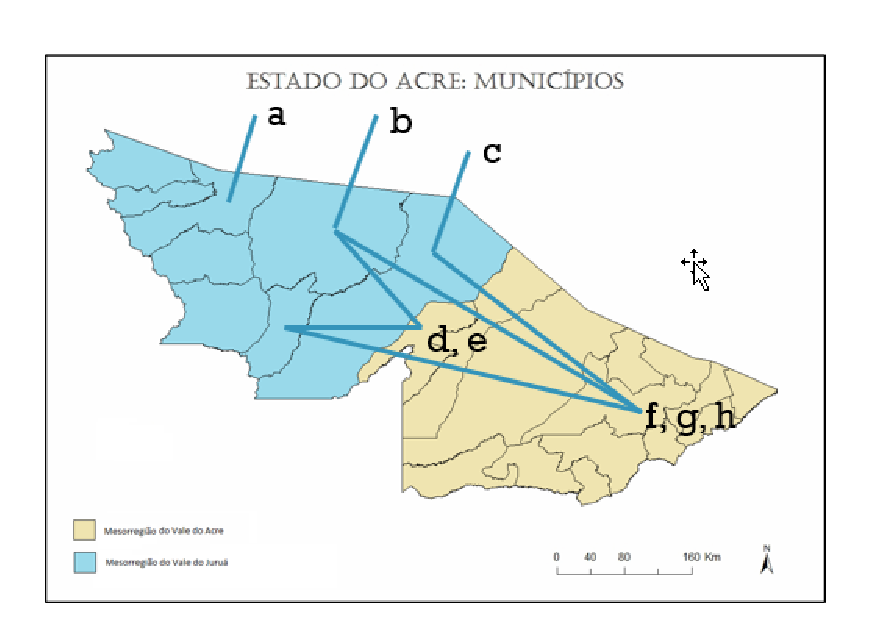
\includegraphics[scale=0.2]{fig1}

\[
W_{blue}=\frac{\left[\begin{array}{ccc}
c_{i1} & \dots & c_{iN}\end{array}\right]}{\sum_{j=1}^{N}c_{ij}}\quad W_{blue}=\frac{\left[\begin{array}{ccc}
5 &  & 3\end{array}\right]}{8}=\left[\begin{array}{cc}
0.625 & 0.375\end{array}\right]
\]

\end{frame}

\section{Data}

\subsection{Database Description}
\begin{frame}{Data}

{\scriptsize{}}%
\begin{tabular}{|>{\raggedright}p{2.5cm}||>{\raggedright}p{1.5cm}||>{\raggedright}p{2cm}||>{\raggedright}p{3cm}|}
\hline 
\textcolor{black}{\footnotesize{}Variable} & \textcolor{black}{\footnotesize{}Source} & \textcolor{black}{\footnotesize{}Frequency} & \textcolor{black}{\footnotesize{}Range}\tabularnewline
\hline 
\textcolor{black}{\footnotesize{}Brazilian Industrial Production} & \textcolor{black}{\footnotesize{}IBGE} & \textcolor{black}{\footnotesize{}Monthly} & \textcolor{black}{\footnotesize{}2004-01 to 2016-12}\tabularnewline
\hline 
\textcolor{black}{\footnotesize{}Employment and Unemployment} & \textcolor{black}{\footnotesize{}CAGED} & \textcolor{black}{\footnotesize{}Monthly} & \textcolor{black}{\footnotesize{}2004-01 to 2016-12}\tabularnewline
\hline 
\textcolor{black}{\footnotesize{}Meso-regions and municipalities} & \textcolor{black}{\footnotesize{}IBGE} & \textcolor{black}{\footnotesize{}N/A} & \textcolor{black}{\footnotesize{}as of 2015}\tabularnewline
\hline 
\textcolor{black}{\footnotesize{}Connecting between regions} & \textcolor{black}{\footnotesize{}IBGE} & \textcolor{black}{\footnotesize{}N/A} & \textcolor{black}{\footnotesize{}as of 2007}\tabularnewline
\hline 
\end{tabular}{\scriptsize\par}
\end{frame}

\begin{frame}{Data}

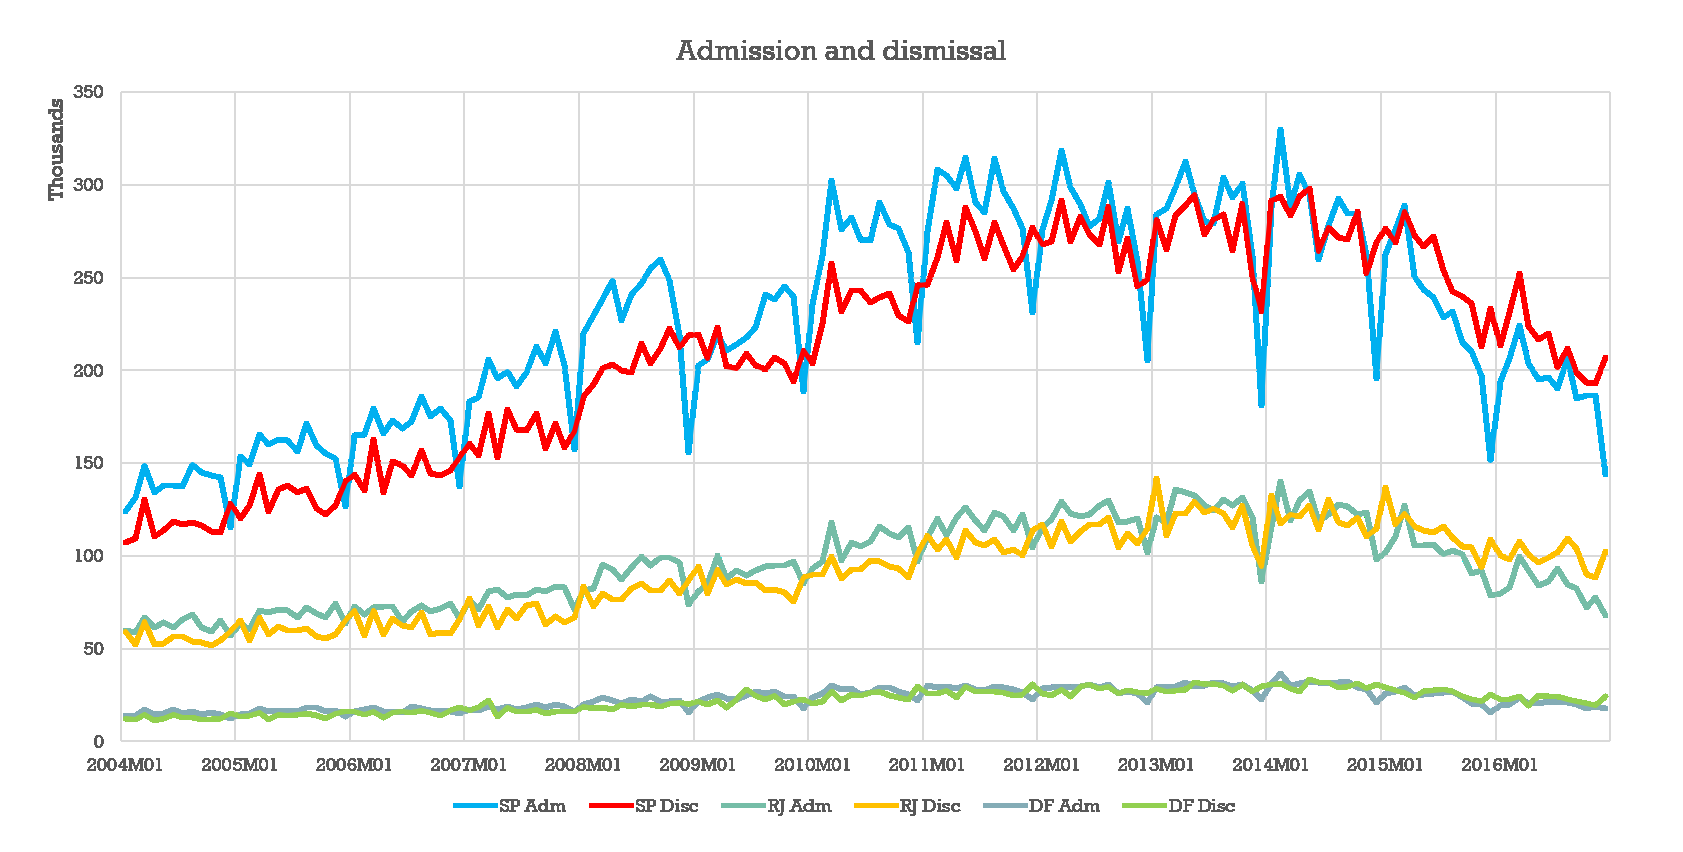
\includegraphics[scale=0.35]{fig2}
\end{frame}


\section{Results}

\subsection{Cumulative Employment}
\begin{frame}{Results}
\begin{itemize}
\item 137 specific models were specified.
\begin{itemize}
\item Domestic variables: 98 models with lag 2 and 39 models with lag 1
\item Foreign variables: 91 models with lag 2 and 46 models with lag 1.
\item 9 models with 1 cointegration relation and 128 models with 2 cointegration
relations.
\end{itemize}
\item Several scenarios were estimated to assess the impact of industrial
production on the labor market.
\begin{itemize}
\item Annual growth of 0\%: A negative employment balance for at least the
next 8 years.
\item Annual growth of 2\%: A positive accumulated balance of 2.5 million
job positions for 8 years ahead.
\item Higher growth scenarios (4\%, 6\% and 8\%) show significant improvements
in the labor market.
\end{itemize}
\end{itemize}
\end{frame}

\begin{frame}{Results}

\includegraphics[scale=0.6]{\string"Figure1 v2\string".eps}
\end{frame}


\subsection{Elasticity}
\begin{frame}{5 major regions}

\begin{itemize}
\item {\footnotesize{}Focusing on the five major regions of Brazil (North,
Northeast, Southeast, South and Central), it was possible to determine
the elasticity of employment in relation to industrial production
for each major region. South (0.18) - North East (0.16) - South East
(0.1) - North (0.06) - Central (0.06)}{\footnotesize\par}
\end{itemize}
{\tiny{}}%
\begin{tabular}{rr}
\includegraphics[scale=0.2]{\string"5major/Figure2-a v2\string".eps} & \includegraphics[scale=0.2]{\string"5major/Figure2-b v2\string".eps}\tabularnewline
\includegraphics[scale=0.2]{\string"5major/Figure2-c v2\string".eps} & \includegraphics[scale=0.2]{\string"5major/Figure2-d v2\string".eps}\tabularnewline
\end{tabular}{\tiny\par}
\end{frame}

\begin{frame}{Southeast states}

\begin{itemize}
\item {\footnotesize{}Analyzing the states of the Southeast we have: Rio
de janeiro (0.19) - Espirito Santo (0.09) - S�o Paulo (0.08) - Minas
Gerais (0.07)}{\footnotesize\par}
\end{itemize}
{\tiny{}}%
\begin{tabular}{rr}
\includegraphics[scale=0.2]{\string"Estados/Figure3-a v2\string".eps} & \includegraphics[scale=0.2]{\string"Estados/Figure3-b v2\string".eps}\tabularnewline
\includegraphics[scale=0.2]{\string"Estados/Figure3-c v2\string".eps} & \includegraphics[scale=0.2]{\string"Estados/Figure3-d v2\string".eps}\tabularnewline
\end{tabular}{\tiny\par}
\end{frame}

\begin{frame}{Meso-regions}

\begin{itemize}
\item {\footnotesize{}The GVAR methodology allows estimation of the elasticity
of each meso-region. Porto Alegre (0.19) - S�o Paulo (0.16) - C. Goi�s
(0.07) - Borborema (0.02) - Jequit. (0.02)}{\footnotesize\par}
\end{itemize}
{\tiny{}}%
\begin{tabular}{rr}
\includegraphics[scale=0.2]{\string"MuncRand/Figure4-a v2\string".eps} & \includegraphics[scale=0.2]{\string"MuncRand/Figure4-b v2\string".eps}\tabularnewline
\includegraphics[scale=0.2]{\string"MuncRand/Figure4-c v2\string".eps} & \includegraphics[scale=0.2]{\string"MuncRand/Figure4-d v2\string".eps}\tabularnewline
\end{tabular}{\tiny\par}
\end{frame}

\begin{frame}{Meso-regions}

\begin{itemize}
\item {\footnotesize{}Elasticity of the most populated meso-regions. Rio
de Janeiro (0.19) - Porto Alegre (0.19) - Belo Horizonte (0.17) -
S�o Paulo (0.16) - C. Goi�s (0.07) - Salvador (0.11)}{\footnotesize\par}
\end{itemize}
{\tiny{}}%
\begin{tabular}{rr}
\includegraphics[scale=0.2]{\string"MuncCapital/Figure5-a v2\string".eps} & \includegraphics[scale=0.2]{\string"MuncCapital/Figure5-b v2\string".eps}\tabularnewline
\includegraphics[scale=0.2]{\string"MuncCapital/Figure5-c v2\string".eps} & \includegraphics[scale=0.2]{\string"MuncCapital/Figure5-d v2\string".eps}\tabularnewline
\end{tabular}{\tiny\par}
\end{frame}

\begin{frame}{Dynamics of the region}

\begin{itemize}
\item VIDEO
\end{itemize}
\end{frame}

\section{Conclusions}
\begin{frame}{Main Conclusions and limitations}
\begin{itemize}
\item The GVAR methodology proved a parsimonious modeling of the labor market
at regional level, (mesoregion) taking into account the external influences
of each region.
\item The model showed the dynamic relationship between the mesoregions,
as well as it was possible to determine the elasticity of the regions.
\item The South, Southeast and Northeast have shown to be very elastic,
presenting a constant interaction in their regions, while the North
and Central regions seem to suffer little influence from the neighboring
regions.
\item Limitations 
\begin{itemize}
\item Small sample of employment series, data availiable only from 2004
onwards.
\item The GVAR toolbox does not currently incorporate dummy variables, or
seasonality analysis.
\end{itemize}
\item Extensions Evaluation of the model taking into account the American
industrial production.
\end{itemize}
\end{frame}

\section{Possible Extensions}
\begin{frame}{Assets and Liabilities returns:}
\begin{itemize}
\item A more comprehensive macroeconomic model can be formulated and different
types of macroeconomic shocks can be identified and their impact simulated.
\item It is possible to construct a \textquotedblleft tailor-made\textquotedblright{}
GVAR. This route was explored by Ericsson and Reisman {[}2012{]} but
not in a regional model.
\item Disagregate data by not only regions but also sectors such as agriculture,
industry and services among others.
\item Another possible path of research consists of evaluating predictive
performance at different aggregate levels and horizons against simple
benchmarks such as random walk or first order autoregressive model.
\end{itemize}
\end{frame}


\appendix

\section*{}

\bibliographystyle{plain}
\bibliography{\string"Modelling Brazilian Regional Formal Labor Market Using Global VAR Approach\string"}

\end{document}
